\documentclass[conference]{IEEEtran}
\IEEEoverridecommandlockouts
% The preceding line is only needed to identify funding in the first footnote. If that is unneeded, please comment it out.
\usepackage{cite}
\usepackage{amsmath,amssymb,amsfonts}
\usepackage{algorithmic}
\usepackage{graphicx}
\usepackage{textcomp}
\usepackage{xcolor}
\def\BibTeX{{\rm B\kern-.05em{\sc i\kern-.025em b}\kern-.08em
    T\kern-.1667em\lower.7ex\hbox{E}\kern-.125emX}}
\begin{document}
\baselineskip=13pt
\title{Economy and energy: are we heading for an asymptote? }

\author{\IEEEauthorblockN{Léa TRIN}
\IEEEauthorblockA{\textbf{Supervisors: } Gregory De Temmerman, Dimitri Chuard \\
{Zenon research}\\
}

}

\maketitle

\begin{abstract}
\baselineskip=13pt
The correlation between global energy consumption and GDP growth, and the challenges of the upcoming energy transition, raises fears of a massive economic downturn in the coming years. In this paper, we study the correlation between primary energy consumption and economic growth for a wide range of countries over time. We show that the evolution of the link between GDP and energy appears to be moving towards a reduction in the dependence of economic growth on energy supply, both country by country but also at global level. We also study the energy and resource impact of a recently proposed decarbonisation scenario of the global energy mix to see if this could be a limitation. 

\end{abstract}


\section{Introduction}
Global economic growth, population growth and rising living standards require energy and natural resources. The production of manufactured goods, services and more generally the creation of capital is entirely dependent on energy and mineral resources. 
\\
Currently, most developed countries continue to experience annual economic growth, i.e. an annual increase in their GDP, although at a rate of a few percent per year. Many countries are also developing, mainly through massive industrialization. The most obvious example is China, but India and Brazil are also experiencing an acceleration of their economies.
\\
While there are signs of a slowdown in developed countries, economic growth in many countries shows no sign of abating and global per capita GDP continues to grow.  It is also to be expected that some less developed countries, such as those in Africa, will experience their own development phase in the coming years.
\\
This global economic growth is accompanied by a steady increase in global primary energy demand. However, as our planet is finite, it seems impossible to imagine a continuous growth in global energy demand. Indeed, even the exploitation of renewable energy sources cannot guarantee a constant growth of the world's energy supply, since they require many resources that are present in finite quantities on our planet and cannot be completely recycled. In addition, the climate emergency will push countries to reduce their consumption of fossil fuels, which currently dominate the global energy mix.
\\
Here we ask, looking at the past, how global energy demand can evolve in the face of constant GDP growth. Can we imagine continued global economic growth without growth in energy supply? Have any countries already experienced this? How does energy demand evolve with economy: are there asymptotes and general trends? Finally, will the radical change in energy mix face limitations, especially in terms of mineral resources and the energy required to extract and process those resources?


\section{Developments in the economy-energy coupling in the world}
\begin{figure*}
    \centering
    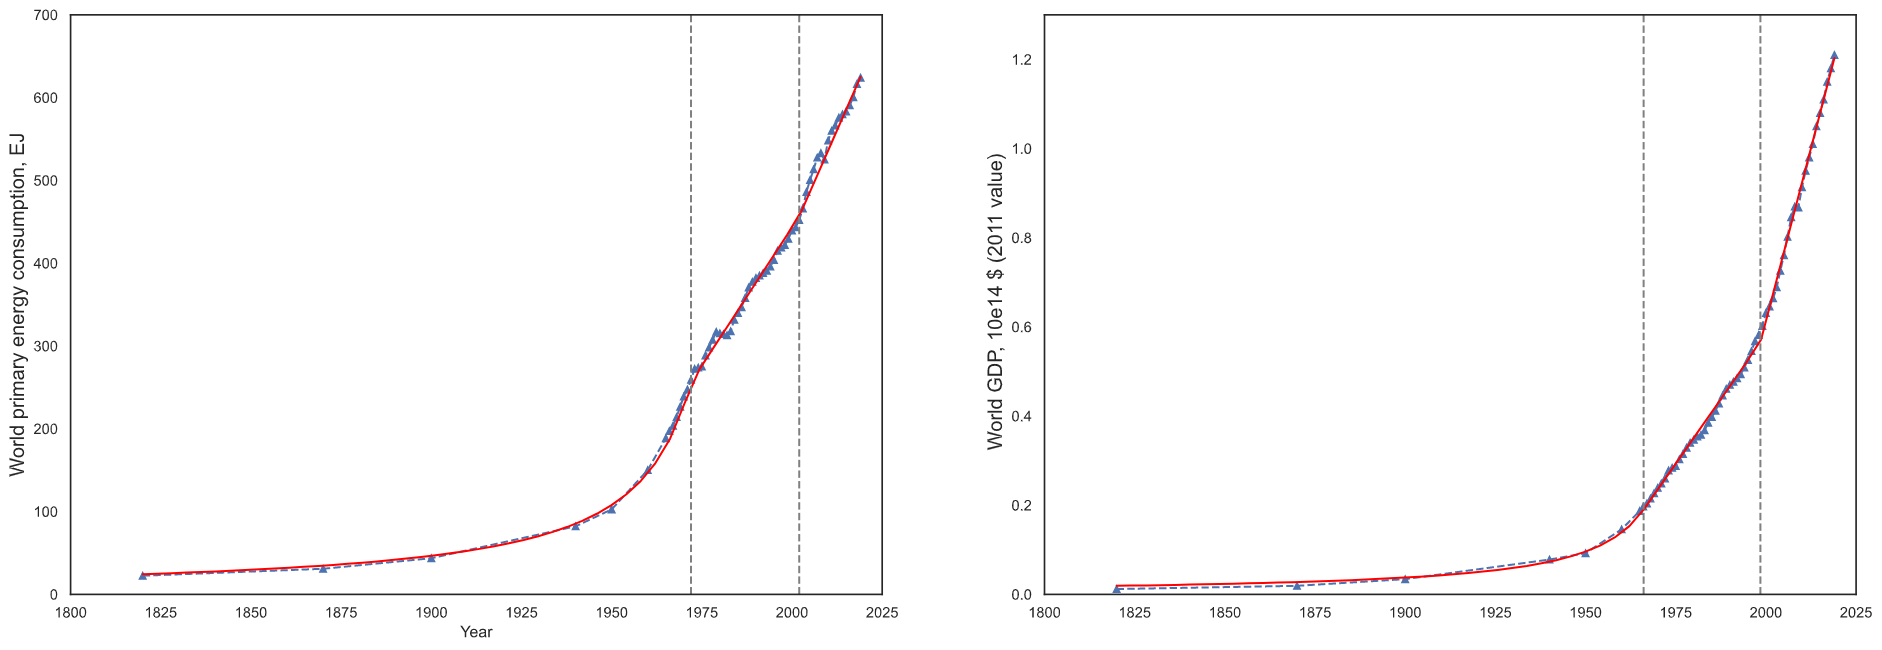
\includegraphics[scale=0.25]{world.png}
    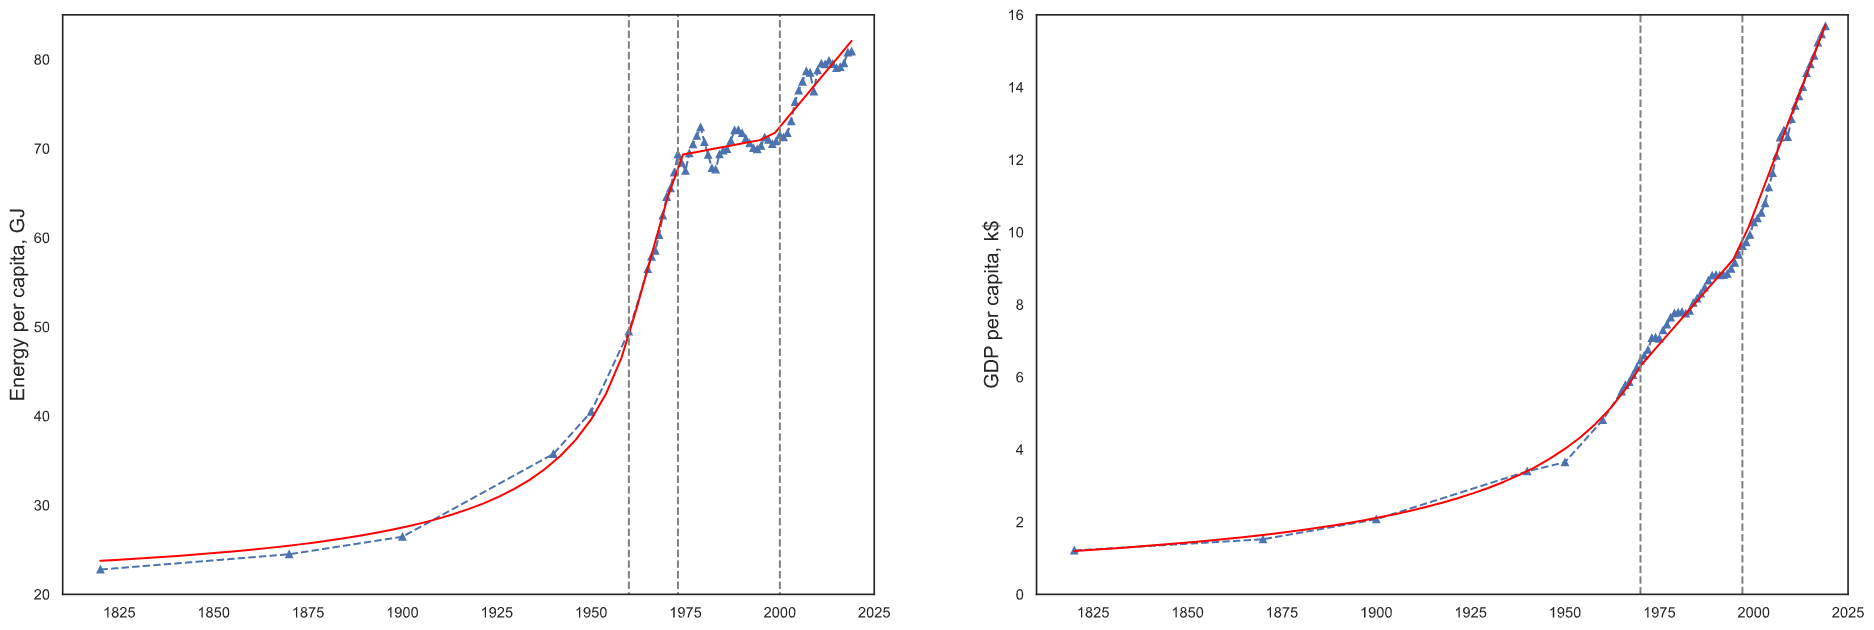
\includegraphics[scale=0.25]{world-percapita.png}
    \caption{World data, GDP data is from the Maddison project \cite{bolt_maddison_2020}, data about primary energy consumption is from BP statistical review \cite{noauthor_statistical_nodate} and population data from \cite{noauthor_history_2020}}
    \label{fig:worlddata}
\end{figure*}
On fig.\ref{fig:worlddata}, we can observe the world GDP per capita since the 19th century. The data is available on the Maddison Project website since time 0 and underlines the fact that the world average incomes remained almost unchanged over a period of several centuries when compared to the increase in incomes over the last 2 centuries. At the beginning of the 19th century, the world experienced a hyperbolic growth until the first oil crisis of the 1970’s. This period was characterized by a strong economic growth and a growth rate which increased every year. 
After the 1970’s, two periods of linear economic growth can be observed. The first one lasted until the beginning of the 21th century and was succeeded by a period of stronger economic growth, which can be linked with the strong growth of the Chinese GDP. Indeed, China's share of world GDP has risen from 3.6\% in 2000 to 17.8 \% in 2019. 
\\
The beginning of the major growth of the world GDP coincides with the first industrial revolution in developed countries. Indeed, this first part was characterized by a strong development in western countries. This development was made possible in part due to the beginning of the exploitation of fossil fuels (mainly coal), which allowed the inhabitants of western countries to produce a larger amount of goods than what they used to produce with the strength of animal and traditional biomass.
\\
Indeed, we can observe that the world primary energy consumption experienced the same phase of hyperbolic growth from the beginning of the 19th century. This period was characterized by a strong industrialization of western countries. Their economy is changing from an agricultural economy to an industrial economy. As energy consumption increases, so does the global GDP. 
But the similarity between the two graphs does not end there, as primary energy demand also entered a linear growth phase in the 1970s and accelerated in the 2000s. This correlation between economy and energy is a well-known fact. Indeed, considering that we transform resources into products and services, and that each transformation requires the use of energy, it seems logical that economic output is related to the amount of energy added used. 
\\
\begin{figure}
    \centering
    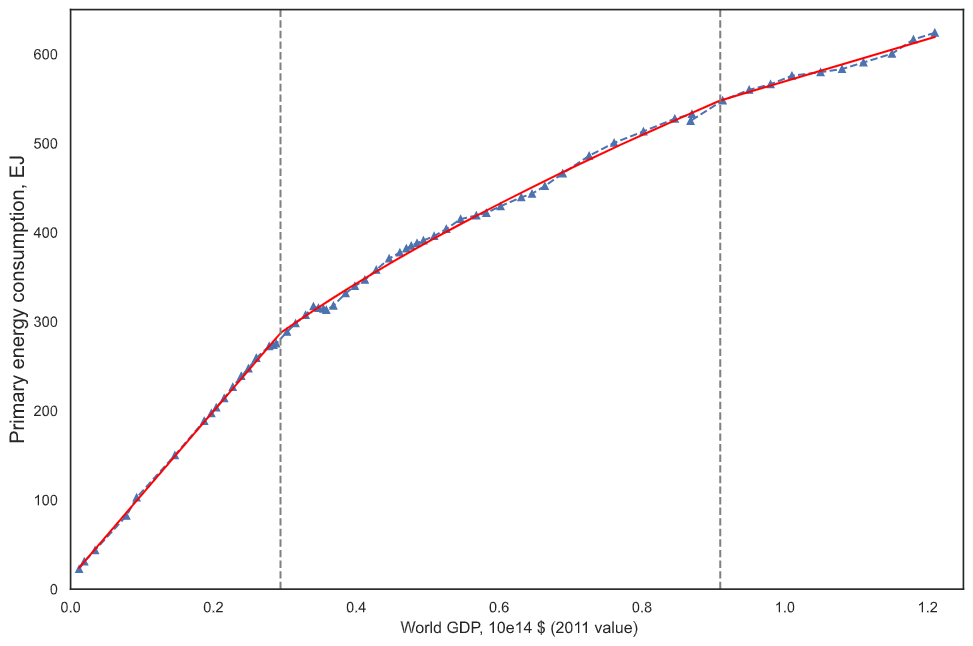
\includegraphics[scale=0.22]{energy-gdp.png}
    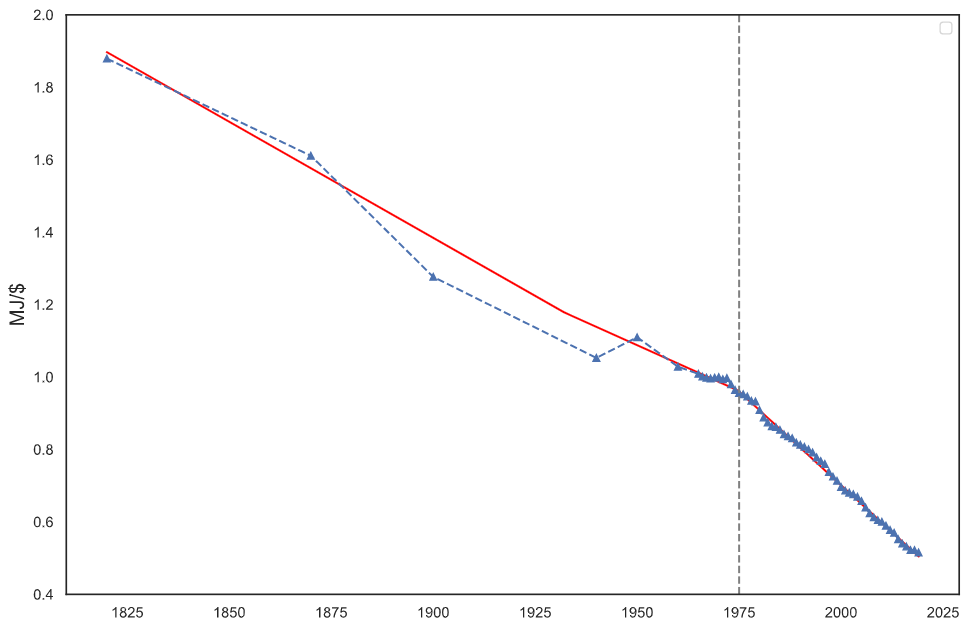
\includegraphics[scale=0.22]{energyint.png}
    \caption{Correlation between GDP and energy consumption, the second graph presents the energy intensity, it means the amount of energy required to produce one GDP unit.}
    \label{worldcorrelation}
\end{figure}
However, this correlation is not constant through time, as we can see on fig.\ref{worldcorrelation}. The economy-energy coupling has also known three different phases. A linear one until the 1970’s, followed by a power model (this fit was chosen because it is often observed in growth mechanism, cf V.Smil, Grotwh) and a new linear period after 2010.
We can see that the coupling between energy and GDP is remarkable but has evolved since 1800 fig 2. It seems that since 1970, the economy has grown faster than the primary energy consumption. This means that the production of one dollar of GDP required less and less energy. Indeed, on fig 1, we can see that the primary energy consumption per capita entered a period of very low growth since 2000 while the GDP per capita continues to increase. 
\\
This observation is a first step towards the idea that economic growth and primary energy consumption can be partially decorrelated. 
To understand this phenomenon, we can express the GDP per capita as follows: 
\begin{equation}
    \frac{GDP}{Population}=\frac{GDP}{Energy Unit}\frac{Energy Unit}{Population}
\end{equation}
Thanks to this identity, we can see that a reduction of the amount of energy required to produce a GDP unit can counterbalance a limitation of energy supply. This kind of reduction can be obtained by reducing the losses in the chain from primary to useful energy. 
This phenomenon of reducing the energy required to produce GDP is clearly observable on a global scale, as we can see on fig 2.  Thus, the observation on the world scale underline that the economy-energy coupling has known 3 main periods, from the beginning of the nineteenth century to the 1970’s, from the 1970’s to the 21st and from the beginning of the century to 2019. These three periods showed a reduction of the amount of energy needed to produce a GDP unit, but they do not prove that a reduction of the energy supply per capita can be offset by the improvement of the energy intensity. Indeed, the energy supply per capita in the world has always increased since the beginning of the 18th century, even if it reached one level in 2015. But this is not the case for all developed countries. 
\\
This is why we will study countries one by one in the second part, to see how the economy-energy coupling has evolved depending on the kind of country. 



\section{Developments in the economy-energy coupling by country} 
In term of economy and energy transition, two types of countries can be defined, depending on the period of their industrialization. V.Smil \cite{smil_energy_2010} describes them as it follows: 
\begin{itemize}
    \item The early innovators, Western Europe and North America which ended the path to a high average per capita energy use during the nineteenth century (or during the eighteenth century for the United Kingdom for instance). 
    \item The late innovators whose dependence on non-fossil energies lasted until the end of the 20th century.
\end{itemize}
	 
Between those two main groups are the countries that began their modernization during the nineteenth century but reached a high development level only during the second part of the 20th century. Japan and Russia are the most concrete examples of this category. 
In this section, we will use data of primary energy consumption and GDP to look at the particularities of each group of countries. Our goal is to detect transition patterns and global trends thanks to national regressions on a various panel of countries. 

\subsection{Formerly industrialized countries}
\subsubsection{Study case: Great Britain} 

\begin{figure}
    \centering
    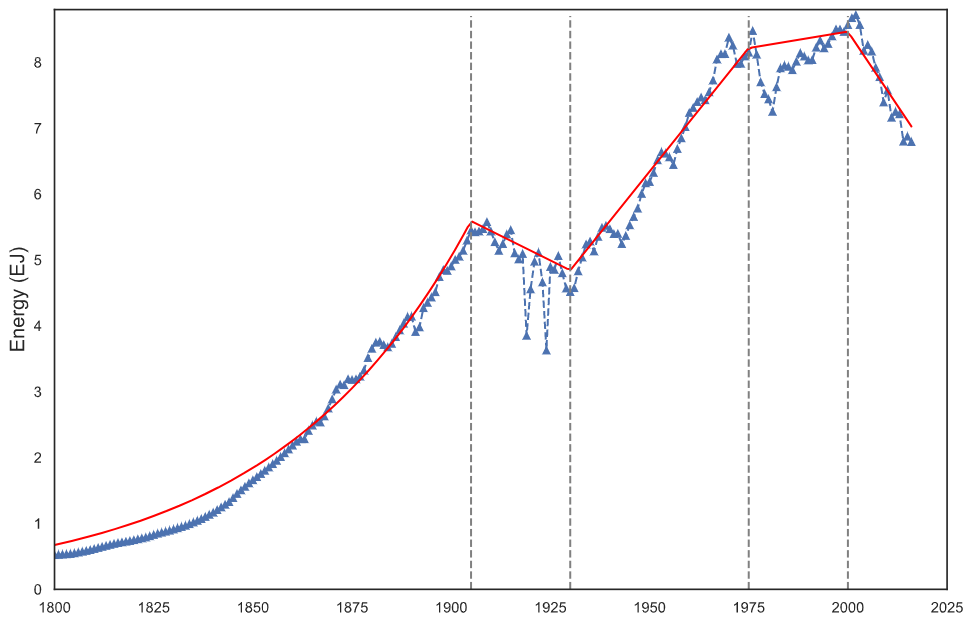
\includegraphics[scale=0.22]{energy-GBR.png}
    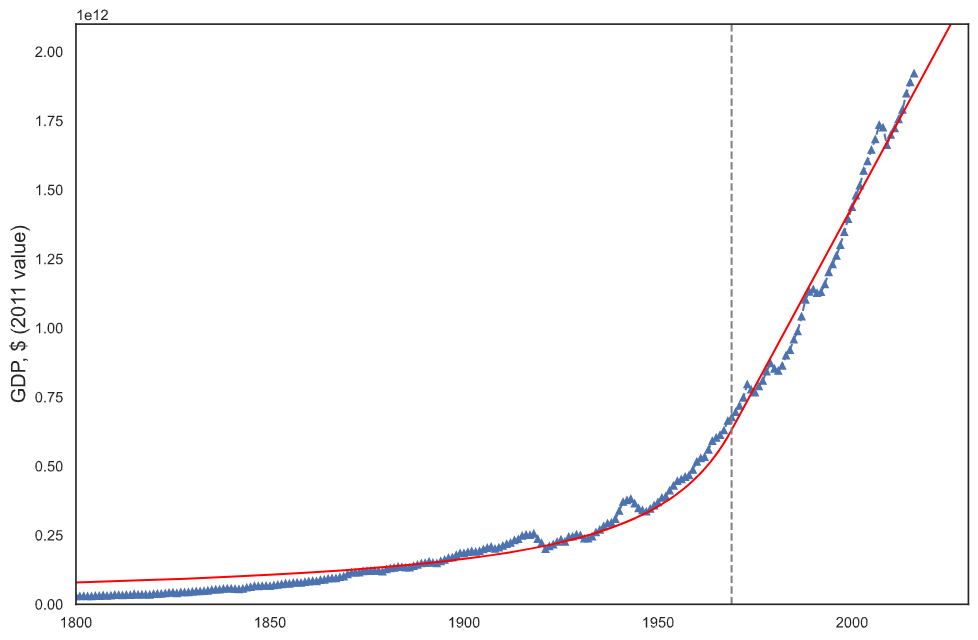
\includegraphics[scale=0.22]{gdp-gbr.png}
    \caption{Energy consumption and GDP evolution of the UK since 1800, data is taken from \cite{harvard_university_national_2021} and \cite{bolt_maddison_2020}}
    \label{GBR}
\end{figure}
Britain was the first country to achieve the energy transition from biomass to coal, more recently it had been a forerunner in nuclear electricity, and it has been a major developer of offshore hydrocarbons. The study of this country, whose energy transition process seems to be ahead of schedule, can therefore give us an initial overview of the different transitions that a country can undergo from its industrialization to the end of its development.
\\
Looking at the two previous graphs on fig.\ref{GBR}, we can do two rapid observations:
\begin{itemize}
    \item The evolution of the primary energy consumption of the UK is much more complex than the global one.
    \item The correlation between energy consumption and the GDP growth is less obvious than it was for the world data.
\end{itemize}
During the 19th century, primary energy consumption has experienced exponential growth. This period of high growth in energy supply can be linked with a period during which coal dominated thermal energy use. All the coal fields were opened since 1640 and the strong economic growth was based on the comfortable coal resources that the country owned \cite{smil_energy_2010}. 
British coal production reached its peak in 1913 (with 287 Mt). This peak is clearly recognizable on the first graph. This peak can be linked with two general strikes in 1921 and 1926. After this, the energy consumption knew a period of decrease, but the UK did not experience a period of economic regression. 
\\
\begin{figure}
    \centering
    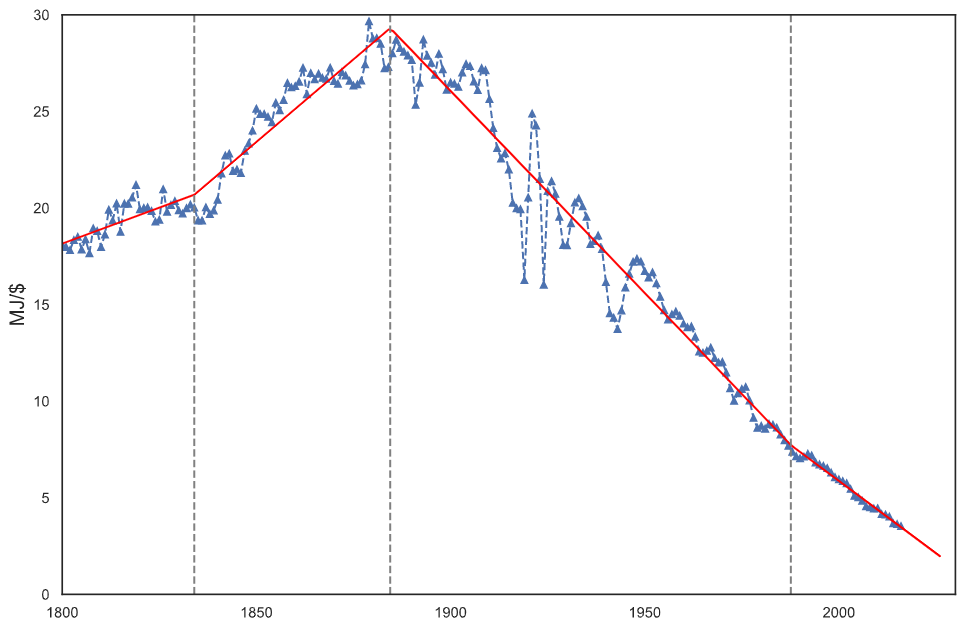
\includegraphics[scale=0.22]{energy-eff-gbr.png}
    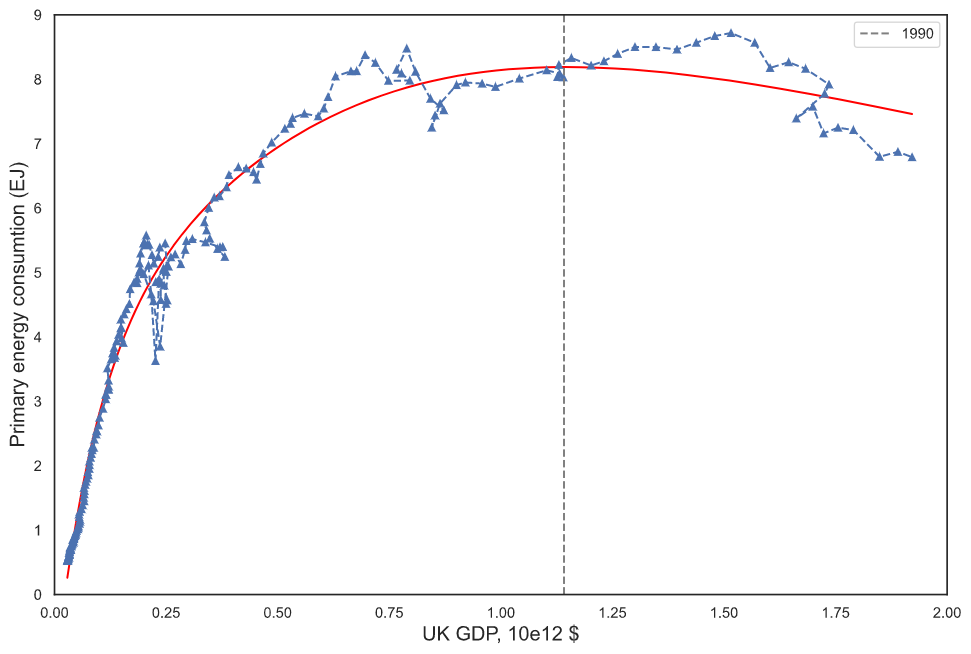
\includegraphics[scale=0.22]{energyintensity-GBR.png}
    \caption{Correlation between energy and GDP for the United Kingdom}
    \label{GBRcorrel}
\end{figure}
Indeed, as we can see on the graph about energy intensity (fig.\ref{GBRcorrel}), the limitation of coal supply pushed the country to improve its energy efficiency. This technological improvement was motivated by economic interests. After this period, energy consumption grew again from 1925 to 1975. During this period, the country consumed more and more natural gas and oil and the strikes of the 1980’s marked the beginning of the end of coal production in the country. 
In 1975, the growth in the energy consumption slowed down as well as the world’s consumption, but the energy supply did not recover and the primary energy consumption of the country began to decrease in 2000, even if the country developed new supply sources. 
\\ 
\\
The growth of the British GDP has known two periods since the beginning of the nineteenth century. During the first one, the growth was hyperbolic, after the 1970’s, the growth became linear and did not change during the 21st century. 
The shift from hyperbolic to linear growth coincides with a slowdown in the growth of energy supply. It is difficult to establish a causal link between the two breaks, unlike the first phase of growth experienced by the United Kingdom in the 17th century and driven mainly by the discovery of coal and the beginning of energy abundance.
\\
What can be retained from the case of the United Kingdom is the country's ability to maintain economic growth despite the decline in their energy supply, first by improving yields (1900-1925) and then by an expansion of the services sector  of the economy (1970- today).  
We shall see that this trend can be observed in most of the formerly industrialized countries.


\subsubsection{Formerly developed countries}

\begin{figure*}
    \centering
    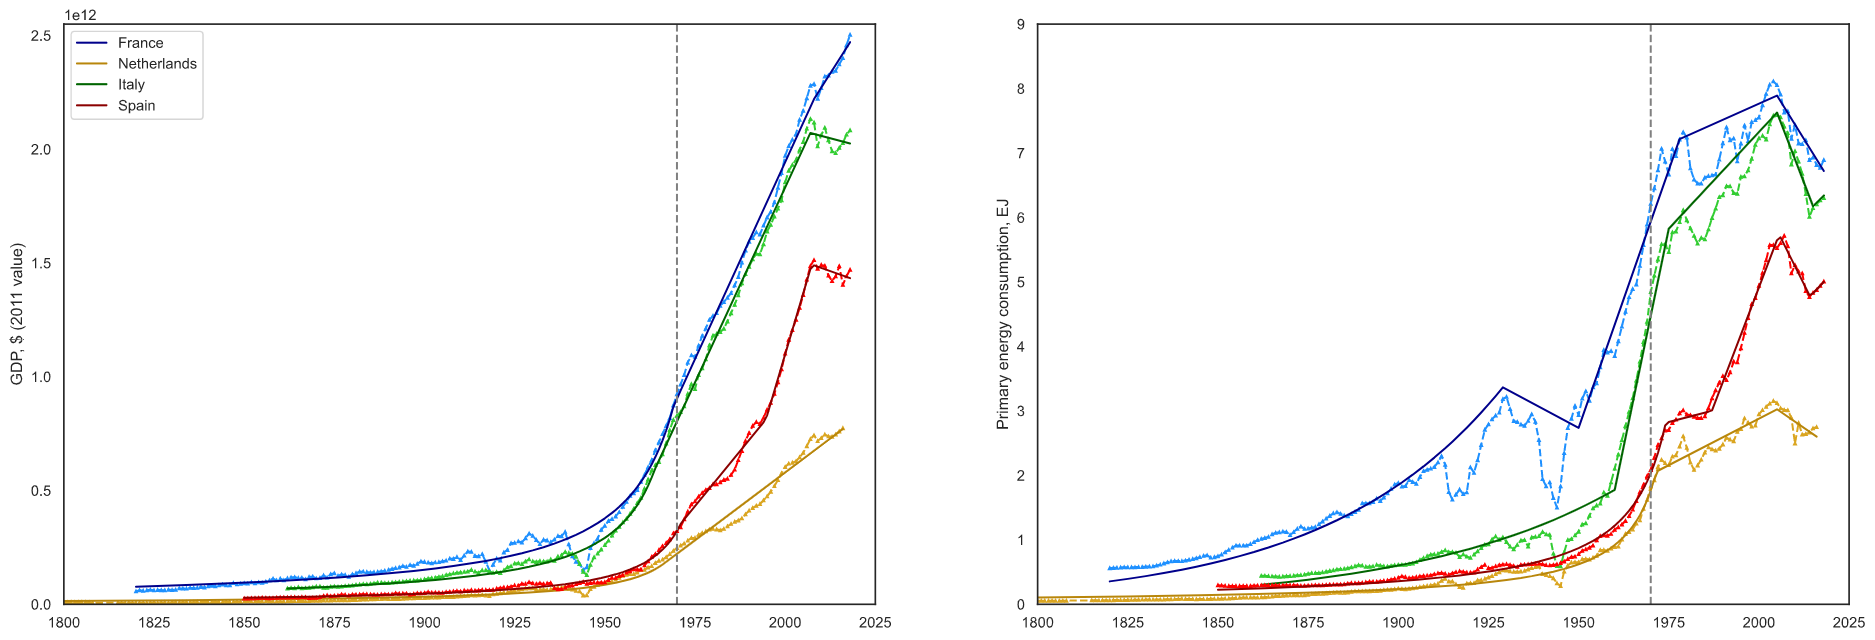
\includegraphics[scale=0.25]{europe.png}
    \caption{Primary energy consumption and GDP of some European countries \cite{harvard_university_national_2021}, \cite{bolt_maddison_2020}}
    \label{europe}
\end{figure*}

The primary energy demand curve for the United Kingdom shows a recurring phenomenon among developed countries: since the 2000s, the primary energy supply of these countries has been stagnating or decreasing. However, the majority of these countries have not experienced a recessionary phase, with the exception of Greece, Spain and Italy for example.
\\
Looking at the primary energy consumption and the GDP evolution of some developed countries, we can see that a shift occurred in both economic growth and energy consumption at the end of the 20th century. The two World Wars, the great depression and the oil crisis produced major changes in these developed economies. 
\\
In the case of the United States, they experienced a short period of recession during WWII and a rapid growth of their energy consumption after 1945. But their economy was severely impacted by the oil crisis in the 70’s. This resulted in a rapid decrease of their primary energy consumption and a circling and twisting curve on figure. 
\\
Oil crisis had a less severe impact on countries with a more independent energy policy. For instance, Japan had a positive economic growth during the second oil crisis because the government increased nuclear and hydropower energy consumption and reduced oil consumption. The same phenomena happened in France whose nuclear program began in the 1950’s. 
Italy is another example as the low impact of the oil crisis on its economy can be linked with its low energy dependency as a result of a service-based industry. 
Thus, the oil crisis and the decrease in primary energy supply can have very different impacts on economies depending on their industry and their energy mix. A contraction in energy supply will not always result in an economic recession. 
\\
\begin{figure}
    \centering
    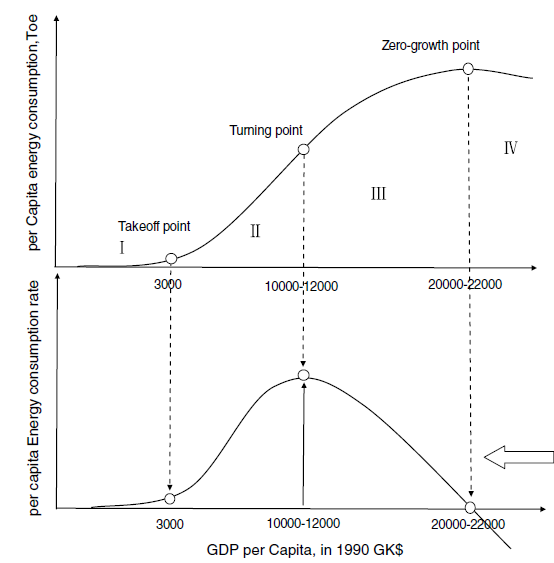
\includegraphics[scale=0.7]{wang.PNG}
    \caption{S-curve Model of Relationship Between Energy
Consumption and Economic Development developed by A.Wang \cite{wang_s-curve_2014}}
    \label{wang}
\end{figure}
On all the developed countries curves, we can observe a period of reduction of the national energy consumption (fig.\ref{europe}). However, we can observe that this reduction does not always fit with a decreasing GDP. The continued growth in GDP per capita is explained by the improvement in the energy efficiency of these countries. In fact, the energy/GDP ratio has decreased for all developed countries (fig.\ref{correldev}). 
This phenomenon can also be seen quite clearly in the last graph of fig.\ref{correldev}, where the quantity of primary energy per capita is plotted as a function of GDP per capita. The curves obtained have the appearance of S curves which can be broken down into 4 phases (fig.\ref{wang}) according to Wang \cite{wang_s-curve_2014}. The first phase (I) is located before the point of detachment, when energy intensity is low and increases little because the majority of the resources exploited are not very energy dense. This corresponds for countries to periods when the majority of the economy is turned towards agriculture. 
The second phase (II) corresponds to a rapid growth in the amount of energy needed to produce one dollar of GDP. More and more energy is needed to produce a dollar of GDP as countries industrialize massively due to the arrival of coal. The abundance of energy and the beginning of innovative technologies explain low yields and therefore high energy consumption for the production of capital. 
The point of inflection of this energy/GDP curve then arrives: the improvement in the yields of the technologies exploited for the massive industrialization of countries explains this inflection. The countries then leave their industrialization phase to enter an era where their economy is already mostly secondary. 
As they continue to develop and exceed 22k\$ of GDP per capita, countries generally enter a phase of tertiarization. This change in the economy explains the entry into a declining phase, as the tertiary economy is much less energy intensive than the secondary one. 
\\
\\
After the 2000s, developed countries therefore began a phase of improving their energy efficiency to allow their economic growth to continue despite the decline in their primary energy supply. For most of these countries, the energy supply per capita stagnates or decreases while the GDP per capita continues to grow. This observation does not take into account energy used to produce agricultural and manufactured goods abroad.
\\
Thus, formerly developed countries have known different phases and have been able to adapt their energy intensity to preserve their economic growth despite the reduction of their energy supply. The reduction of their energy intensity is mainly due to the emergence of a service based economy. Agriculture and industries which supply these developed countries are now located in developing countries. 
\\
In the next part, we will look at the evolution of the economy and energy consumption of this kind of country to see if their development follows the same path as the one of developed countries. 
\begin{figure}
    \centering
    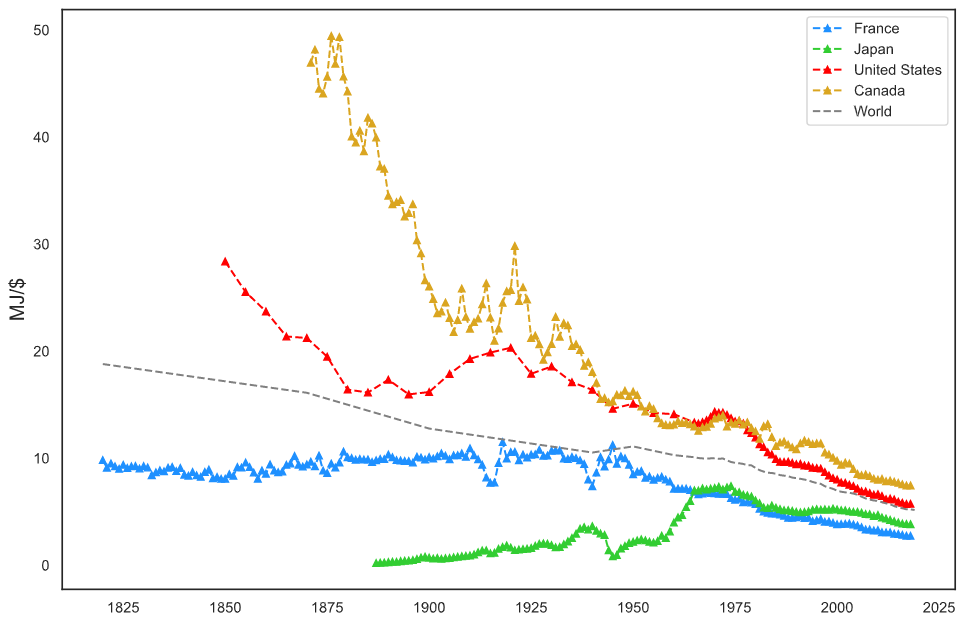
\includegraphics[scale = 0.23]{dev-int.png}
    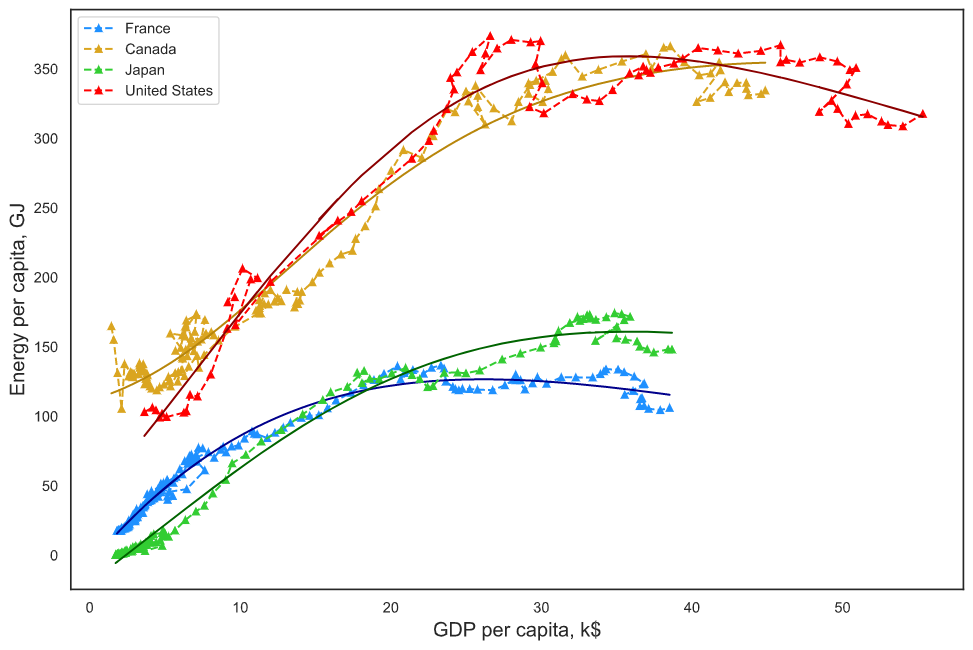
\includegraphics[scale = 0.23]{s-curve-dev.png}
    \caption{Energy and GDP correlation for a panel of developed countries,\cite{bolt_maddison_2020} \cite{harvard_university_national_2021} \cite{noauthor_statistical_nodate} \cite{noauthor_annual_2009} }
    \label{correldev}
\end{figure}

\subsection{Emerging countries}
We are now looking at the case of emerging countries. For this category, we could not find data about primary energy consumption before 1950. Thus, we will focus on the period from 1950 to 2019. Some interesting patterns can be observed during this period as the development of these countries is more recent and some of them seem to display accelerated phases of development.

\subsubsection{Study case: China}
Historically, China was one of the world's largest economic powers for most of the two millennia from the 1st until the 19th century. China’s GDP represented more than one quarter of the global GDP until the end of the 18th century and the industrial revolution of western Europe and north America. China's GDP in 1820 was six times as large as Britain's, the largest economy in Europe \cite{bolt_maddison_2020}. 
Its dependence on non-fossil energies lasted until the second half 20th century.  In 1978, China’s government began its reforms to develop the country and take back its rank of economic leader.  As a result, China has the world's fastest-growing economy, with growth rates averaging 10\% over 30 years. 
\\
\\
\begin{figure}
    \centering
    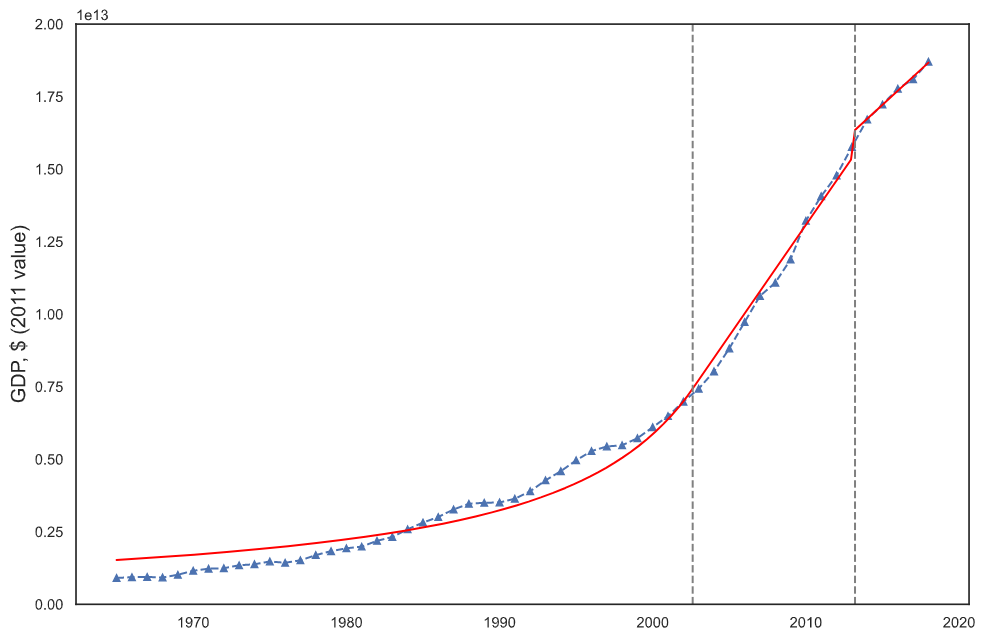
\includegraphics[scale=0.225]{GDP-time-china.png}
    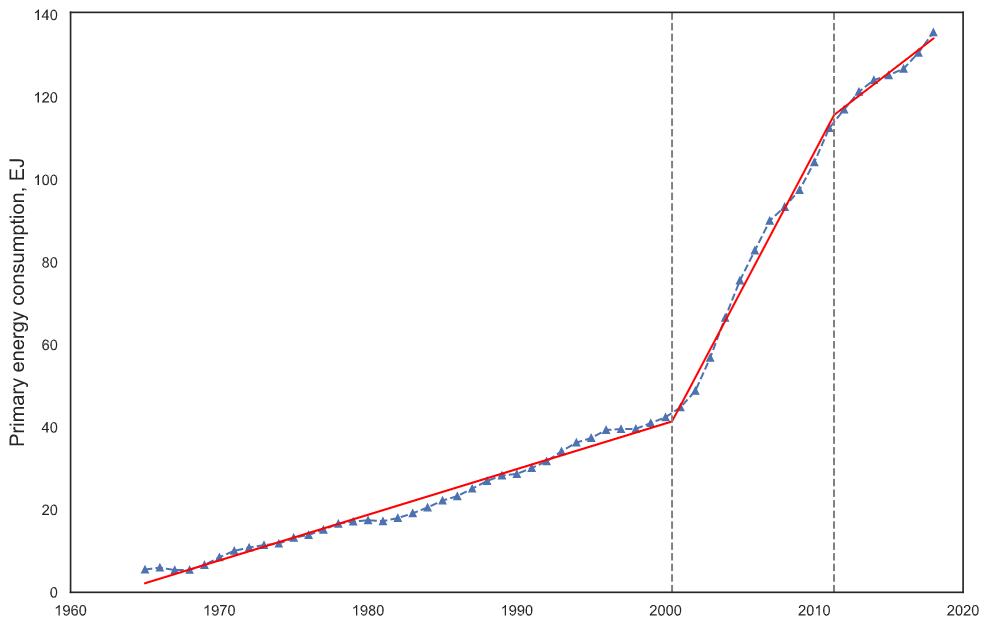
\includegraphics[scale=0.225]{primary-energy-time-china.png}
    \caption{Evolution of China's GDP and primary energy consumption, \cite{bolt_maddison_2020}\cite{noauthor_statistical_nodate}}
    \label{china}
\end{figure}
Looking at fig.\ref{china} we can see that the economy picked up at the beginning of the 20th century as well as the primary energy consumption. But the economic growth and the growth in energy supply slowed down since 2010.  While the causes of this slowdown are manifold and will not be explained here, it can be seen that both the country's economy and its energy consumption tend to flatten out over time, just as the economies of the already developed countries have done.
Looking at the data for China and the countries that developed earlier, we can expect a continuation of this slowdown and a more pronounced decrease in the country's energy intensity in the coming decades. Similarly, the observation of the graph of energy per capita vs. GDP per capita may suggest an evolution along the S-curves of the A.Wang model and a possible entrance in a post-industrialized period. 
Another observation is that the energy intensity of the country has not decreased as much as the one of developed countries. This underlines the fact that China’s economy is still mainly based upon industry. 
\begin{figure}
    \centering
    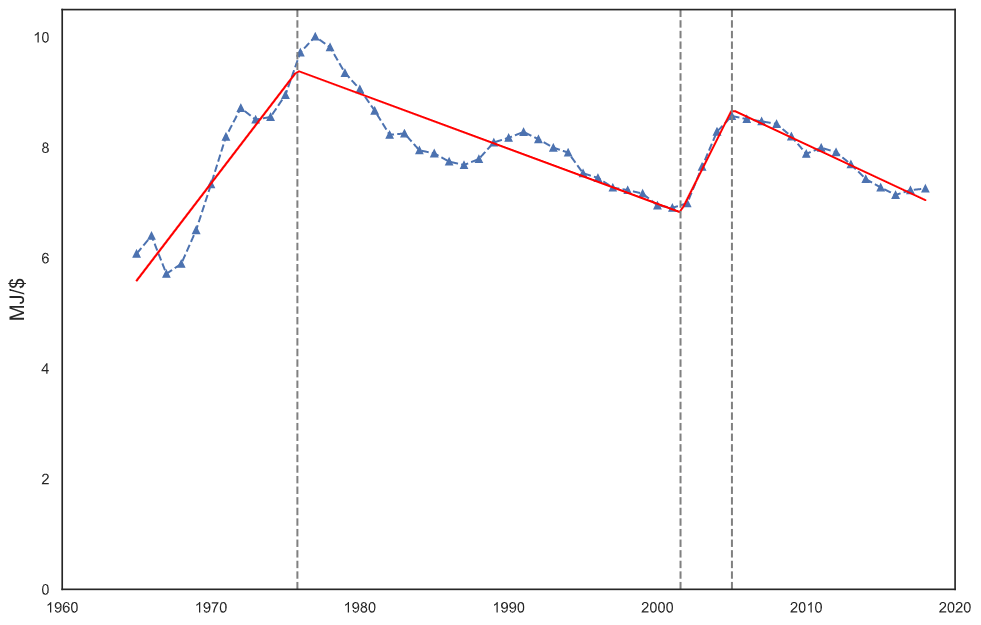
\includegraphics[scale=0.225]{energy-intensity-time-ch.png}
    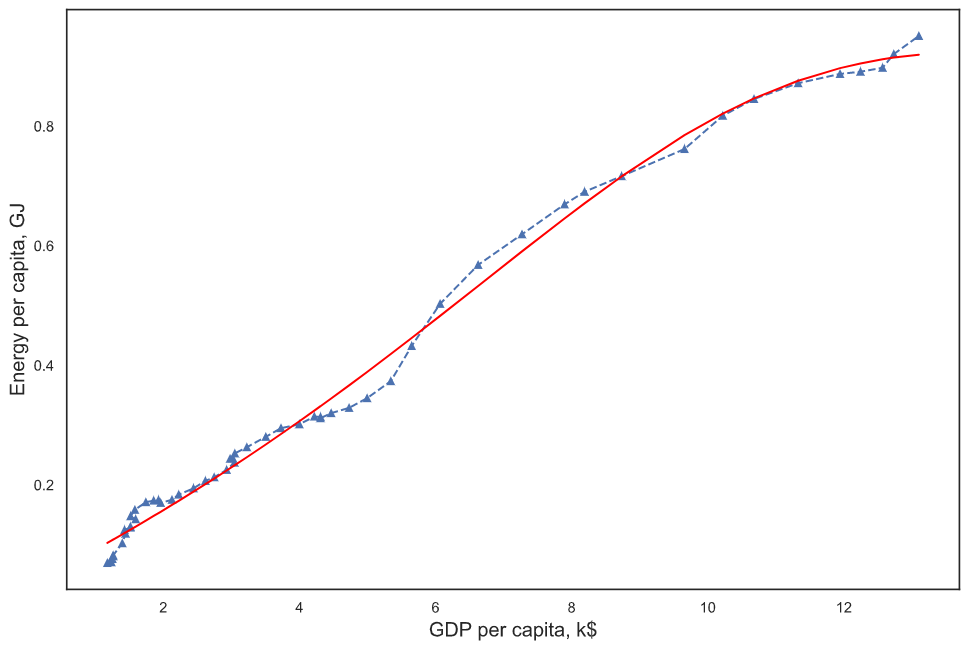
\includegraphics[scale=0.224]{energyc-gdpc-chn.png}
    \caption{Correlation between GDP and energy in China}
    \label{fig:my_label}
\end{figure}
\subsubsection{Overview of the situation in some emerging countries}

In the last section, we look at China which is probably the emerging country in the most advanced stage of development. Now, we will have a look at the case of emerging countries in a less advanced stage of development: India, Brazil, Indonesia and Mexico. 
We can observe that the S-Curve model designed and analyzed by A.Wang in the case of developed countries matches with the model of emerging economies. Most of them have known their inflexion point during the 1990’s while their industrialization began in the 1970’s. 
Some of them as India and Mexico have followed an almost perfect S-curve and seem to approach the zero-growth point. The energy intensity of these countries is way higher than the one of developed countries but has entered a decreasing phase at the same period. 

Thus, observing the historical data of developed and emerging countries, we can see that the development of the countries implies a decreasing energy intensity. All those countries seem to follow a S-Curve trajectory as the one described by A.Wang. There is no guarantee that developments in emerging countries will continue this pattern. However, the similarities observed with already developed countries suggest that this is a serious possibility. 
\\
This can be observed on the global trend as the world energy intensity decreases as well. These observations may suggest that the world energy intensity will continue to decrease and that the correlation between global energy and capita will also follow the path of all these countries and reach a plateau. However, the plateau already observed country by country does not take into account the energy consumed for the non-domestic production of manufactured goods. 
Moreover, this hypothesis could be counterbalanced by the possible development of actual Less Developed Countries’s such as African countries which have not known industrialization yet, but which could follow very different path as their development may not be based on massive use of fossil energies. 
\begin{figure}
    \centering
    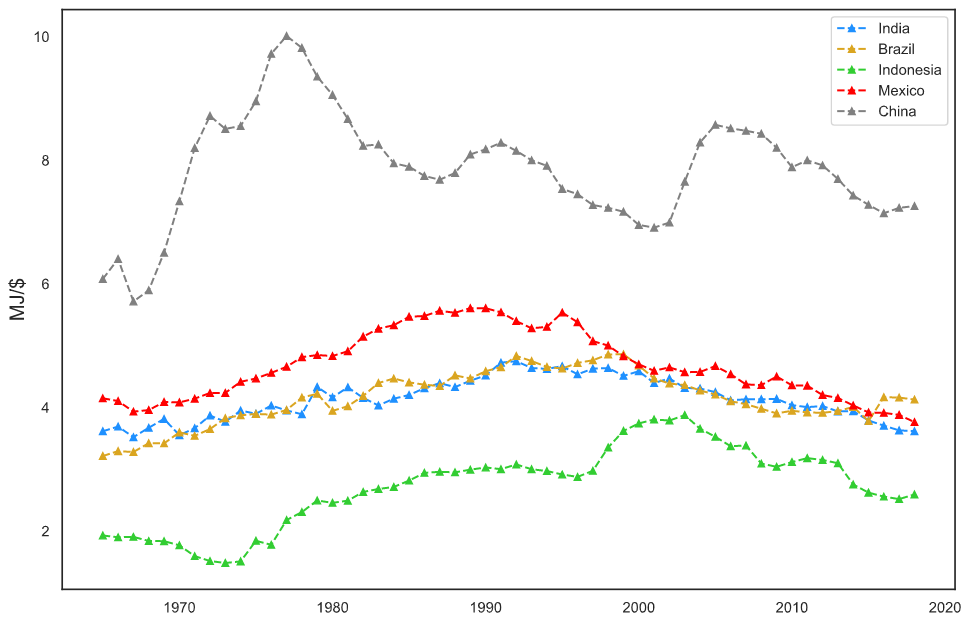
\includegraphics[scale=0.225]{energy-intensity-emerging.png}
    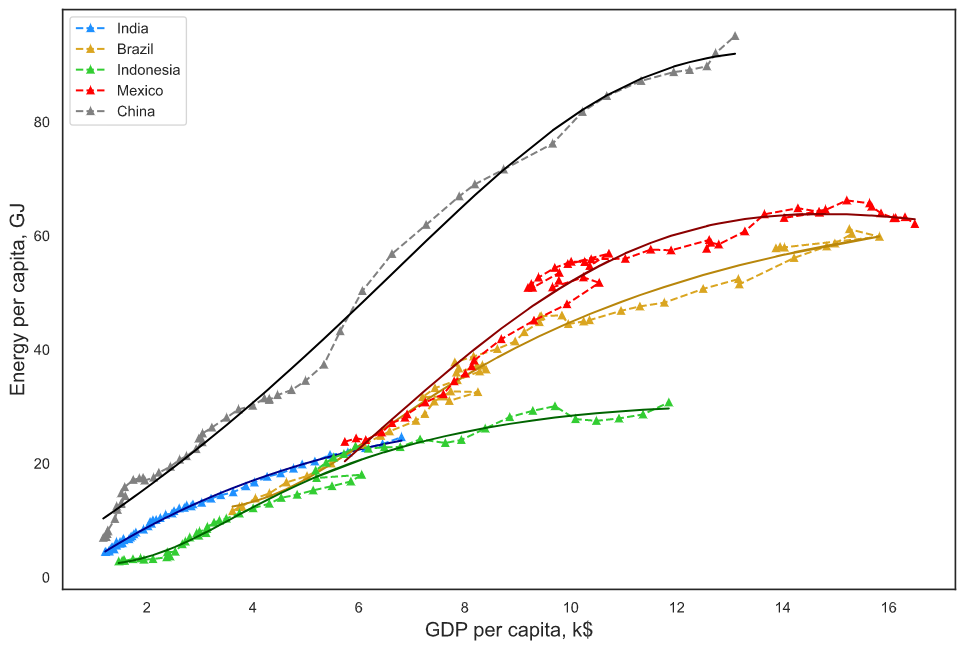
\includegraphics[scale=0.225]{s-curve-emerging.png}
    \caption{Correlation between GDP and energy for emerging countries, \cite{bolt_maddison_2020} \cite{noauthor_statistical_nodate} }
    \label{fig:my_label}
\end{figure}

\section{Development and use of mineral resources: the energy challenge}
If a country's development means increasing energy consumption, it also means increasing consumption of resources such as concrete, steel or copper. Moreover, the energy transition required to cut global greenhouse gas emissions and to offset the decline in fossil fuel supply is often accused of being more mineral-intensive. 
\\
As these mineral resources require considerable energy for their extraction and refining, it is questionable whether it will be possible to achieve the zero-carbon energy system envisaged by the IEA for example \cite{noauthor_net_2021}. 
\\
In this section, we will therefore first examine the energy impact caused by the extraction and refining of mineral resources and how the demand for these resources could evolve with the development of giants such as China. 
Then, we will analyze the excess demand for mineral resources that could be caused by the transition to a zero-carbon energy mix. 

\subsection{Resource demand and economic growth}
% Please add the following required packages to your document preamble:
% \usepackage{booktabs}
\begin{table}[]

\begin{tabular}{cccc}
Commodity  & Consumption (Mt) & Mass Energy need (GJ/t) & Energy need (EJ) \\
Al       & 64.34            & 190                & 12.22            \\
Sb       & 0.14             & 140                & 0.02             \\
Co       & 0.12             & 130                & 0.02             \\
Cu       & 20.98            & 30                 & 0.63             \\
Dy       & 0.00             & 4154               & 0.01             \\
Steel    & 1800.00          & 20                 & 36.00            \\
Li       & 0.04             & 380                & 0.02             \\
Ag       & 0.02             & 1500               & 0.04             \\
Si       & 8.41             & 1000               & 8.41             \\
Ni       & 2.53             & 180                & 0.46             \\
Concrete & 460.00           & 5.6                & 2.58             \\
Fe       & 1.10             & 20                 & 0.02            
\end{tabular}


\caption{Overview of the energy consumption for commodity production by year \cite{vidal_matieres_2018} and various sources for the consumption}
\label{tableun}
\end{table}
The extraction and refining of mineral raw materials essential to the industrial development of countries (e.g. steel, cement, copper) requires considerable energy. While values can vary considerably depending on the extraction and refining processes, the International Energy Outlook (2013) \cite{noauthor_international_2013} estimates that 22\% of the energy consumed by industry is used for steel and cement production alone.
\\
Using OECD sources for the quantities produced and the O.Vidal report for the amount of energy needed to produce certain raw materials, it can be seen that the selection of raw materials presented in table \ref{tableun} alone requires 60 EJ of energy annually, whereas world energy consumption is estimated at EJ by the IEA. 
\\
The extraction and refining of raw materials are therefore already major items of energy consumption in the world. Moreover, during their development, countries consume an increasingly large share of these resources. Indeed, AUTHORS underline that a strong correlation exists between GDP per capita and the annual domestic consumption of commodities such as steel and concrete. This correlation consists in a linear one at the beginning of the development and then a plateau \cite{bleischwitz_extrapolation_2018}. However, there is no sign of decrease in this annual consumption even in formerly developed countries. Thus, we can estimate the rise in consumption of some commodities caused by the development of emerging countries. Using analysis and observations of Bleischiwtz and Nechifor \cite{bleischwitz_extrapolation_2018}, scenarios about economic growth and population growth of the UNO \cite{noauthor_oecd_2021}\cite{noauthor_2019_2019} and the OECD, we can obtain a rough estimate of how the resources consumption could evolve in some emerging countries (fig.\ref{alupr}). The details about the model are given in the appendix. 
\\
This major item of energy expenditure does not therefore seem likely to stagnate or decrease if the GDP per person in households of giants such as India or China continues to grow. 
\\
Moreover, the reduction of our greenhouse gas emissions as well as the reduction of our fossil fuel resources require to transform our energetic system. A new energy mix mainly based on renewable energy and a transportation sector based on electric cars will require a larger amount of metals supply. We will look at this new demand in the next section in order to estimate its impact. 
\begin{figure}
    \centering
    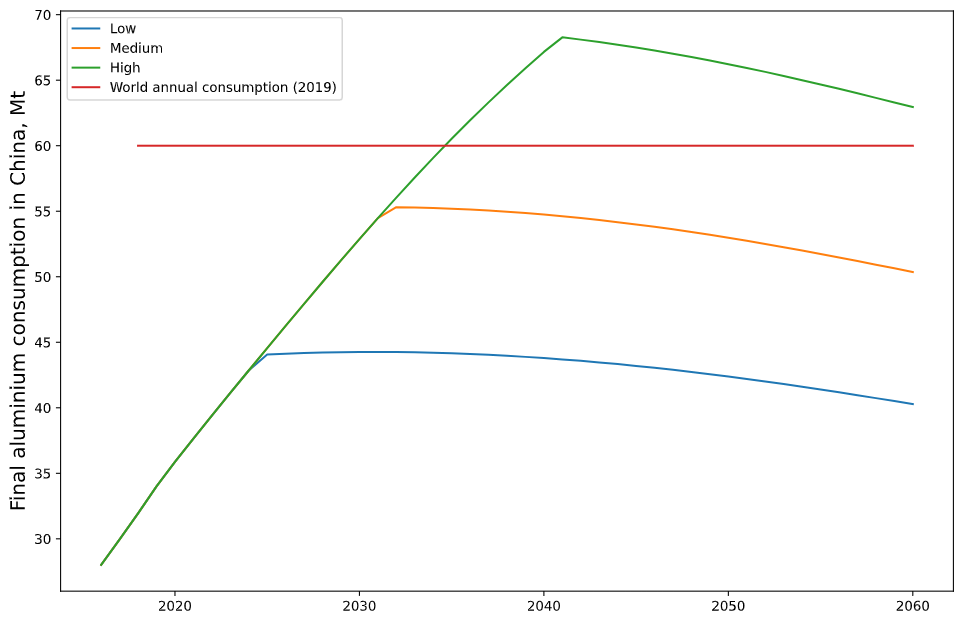
\includegraphics[scale=0.22]{alu-china.png}
    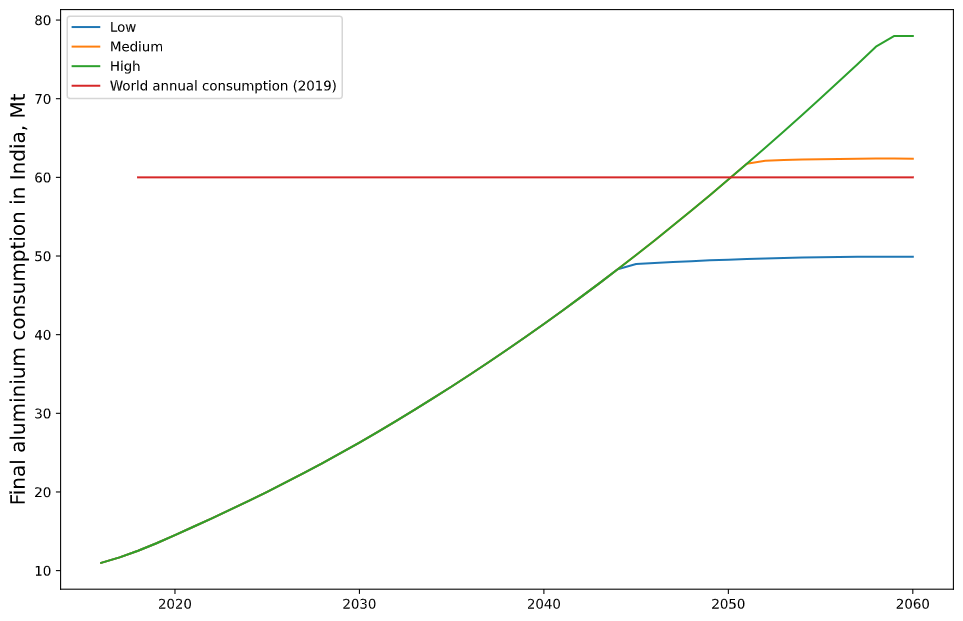
\includegraphics[scale=0.22]{alu-india.png}
    \caption{Scenarios of Aluminium consumption in India and China}
    \label{alupr}
\end{figure}

    

\begin{table*}[]
\begin{center}
\begin{tabular}{lllllllllll}
          & Oil & Coal & Natural gas & Nuclear & Biomass & Hydro & Wind (onshore) & Wind (offshore) & Solar &  \\
Aluminium & 1   & 1    & 2           & 1       & 1       & 0     & 5              & 5               & 40    &  \\
Steel     & 50  & 50   & 80          & 25      & 50      & 25    & 150            & 300             & 175   &  \\
Concrete  & 10  & 10   & 10          & 15      & 1       & 7500  & 500            & 700             & 1100  &  \\
Silicium  & 0   & 0    & 0           & 0       & 0       & 0     & 0              & 0               & 6     &  \\

\end{tabular}
\caption{Estimation of the energy necessary by technology, t/MW \cite{vidal_matieres_2018} }
\end{center}
\end{table*}
\subsection{Energy transition and mineral resources}
Batteries, wind turbines and solar panels are the technologies planned to achieve a zero-carbon energy transition. However, these technologies are often criticized because they require numerous and sometimes critical mineral resources (e.g. rare earths, cobalt, indium). This section looks at the environmental impact of extracting and refining the resources needed for a zero-carbon transition, in terms of the volume of raw material to be extracted from the ground and the energy required to extract and refine these resources. 
\\
Further work could be proposed on the amount of resources needed for the transition scenarios in relation to the resources available on earth. 

\subsubsection{Amount of resources to be extracted from the soil}
The importance of mining activities on a territory can be measured using the Total Material Requirement (TMR) which captures both used and unused resources extracted to produce a final commodity. This indicator can be used to reckon the environmental impact of mining industries at different scales \cite{watari_sustainable_2021}. 
\\
In \cite{bleischwitz_extrapolation_2018}, the authors establish the TMR of resources which will be needed to achieve a decarbonization of the transport and energy industries. They underline that the TMR represented by metal resources is bound to increase from 1 Gt/year in 2015 to 9 Gt/year in 2050 for the electricity sector and from 2 Gt/year to 13 Gt/year in the transport sector. This increase in the volume of material extracted for metals production is often pointed at when dealing with decarbonization of electricity and transport. However, if we compare it with the decrease of the non-metal TMR, we can observe that the total material extracted for the earth ground will be reduced from 58 Gt/year to 39 Gt/year for the aggregated electricity and transportation industry \cite{watari_sustainable_2021}. 
\\
Thus, as the amount of fossil fuel extracted from the ground will be reduced, the quantity of material extracted from our planet may be reduced by the decarbonization of transport and electricity according to Watari \cite{watari_sustainable_2021}. However, the metal material is often more energy intensive. It is therefore interesting to analyze the evolution of the amount of energy required for the installations of energy production in a zero-carbon scenario. This is what will be done in the next section. 

\subsubsection{Net-Zero 2050: What resource and energy needs?}

\begin{figure}
    \centering
    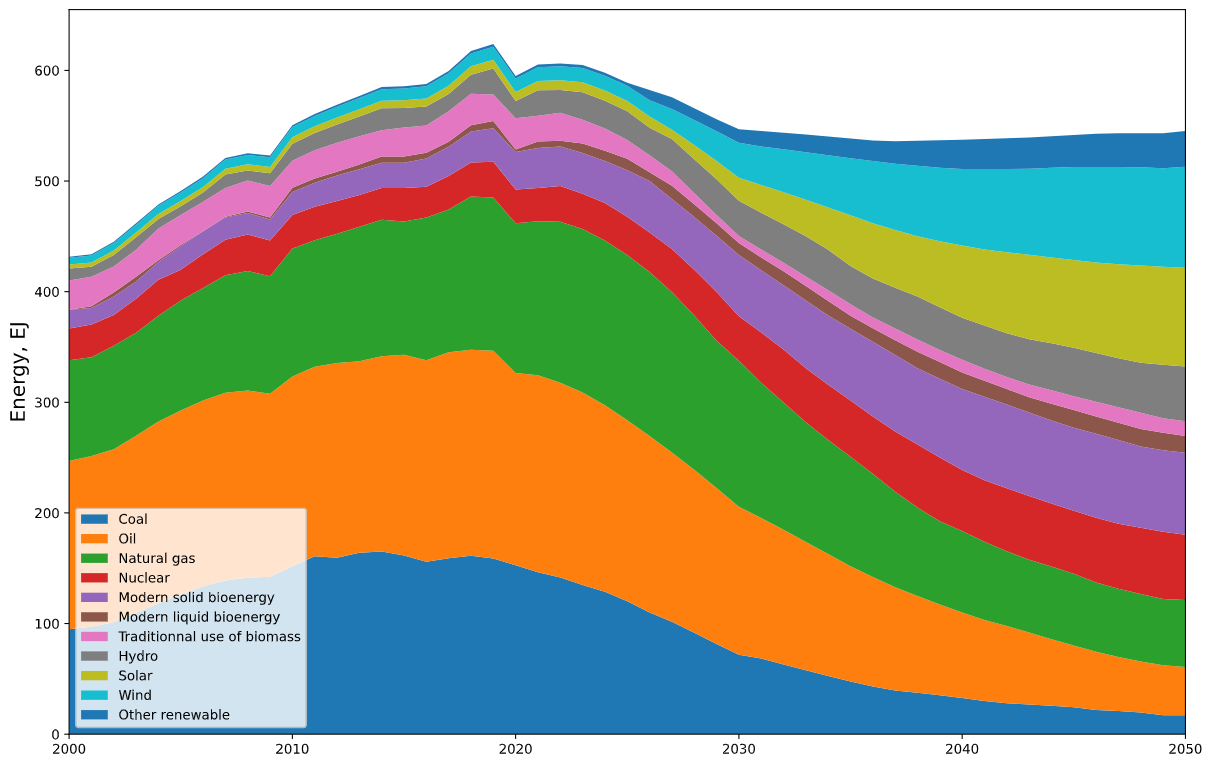
\includegraphics[scale=0.2]{energy-demand-scenario.png}
    \caption{Total energy supply in the Net Zero Emissions 2050 (NZE) \cite{noauthor_net_2021} }
    \label{netzero}
\end{figure}
The IEA recently published a report as a guide to decarbonizing energy by 2050.In this report, they present an energy mix which would allow a carbon-neutrality in energy production (fig.\ref{netzero})\cite{noauthor_net_2021}. This scenario is much more diversified than the actual mix and plan a strong increase in the share of wind and solar power in the global energy mix. However, as we can see in table II, the amount of concrete, steel and copper required to produce energy with this kind of source is much higher than with gas, coal or oil. \\
Thus, using table I and II and the AIE scenario, we can predict the amount of steel, concrete, silicon and aluminum required to achieve this energy mix. The results obtained are given on fig. and the details of the model are given on appendix. The choice of these 4 raw materials is based on table. These commodities are indeed the ones which represents the higher energy consumption for their extraction and production.\\
\begin{figure*}
    \centering
    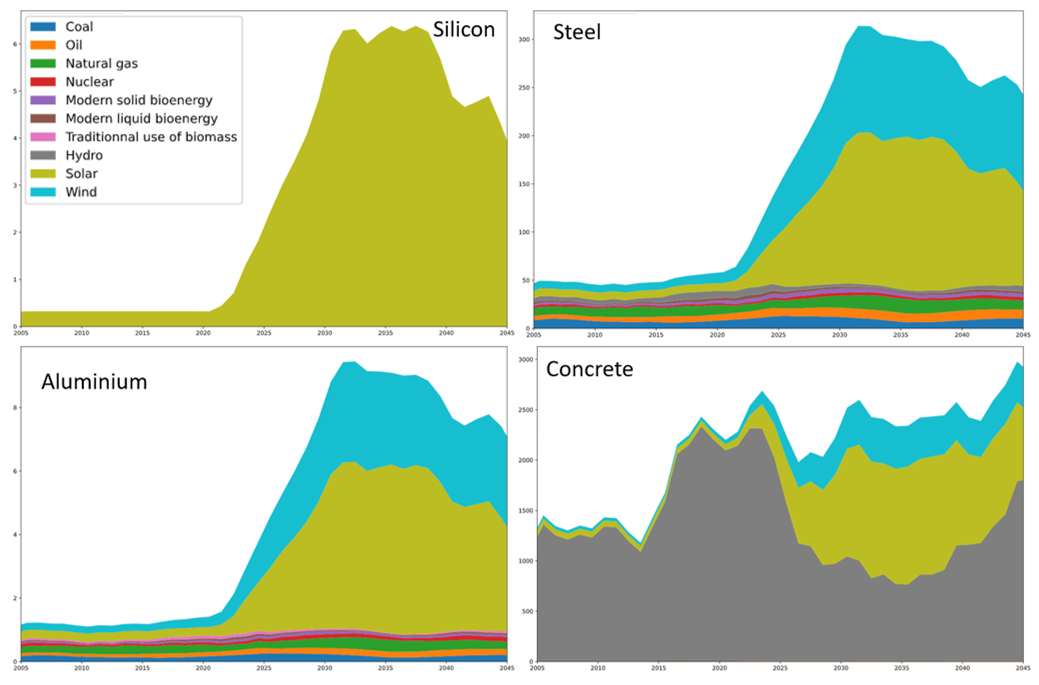
\includegraphics[scale=0.65]{massscen.png}
    \caption{Mass (Mt) of each material required to produce the infrastructures of the NZE scenario}
    \label{massnze}
\end{figure*}
The projections upon the material consumption (fig.\ref{massnze}) of these technologies allowed us to obtain an estimate of the amount of energy required to produce the infrastructures (without the manufacturing cost) of this energy mix (fig.\ref{energynze}). 
\begin{figure}
    \centering
    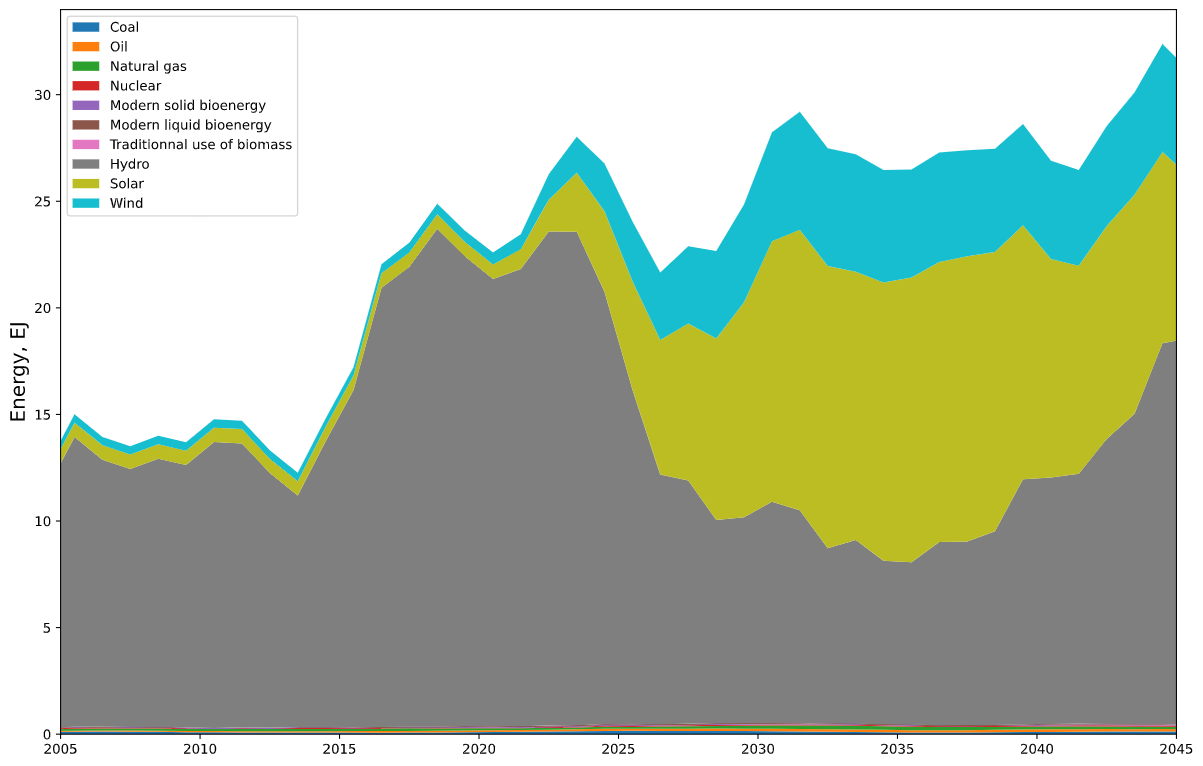
\includegraphics[scale=0.2]{energy-time.png}
    \caption{Energy required for the production of steel, silicon concrete and aluminium by technology following the NZE scenario.}
    \label{energynze}
\end{figure}
Although this estimate is rather rough, it gives an order of magnitude of what can be expected in terms of the energy needed to implement the infrastructures envisaged by the IEA scenario. It can be seen that this energy does not exceed 30 EJ. This number may surpass 25 EJ in 2030 and remain higher than this limit for at least 10 years. Furthermore, this scenario reckons that the primary energy consumption will not continue to grow after 2020. Thus this energetic cost may represent between 5 and 6\% of a global demand in which the rise in consumption of some emerging countries will have to be offset by a reduction of the energy supply of other countries. \\
It is important to note that this number does not take into account all the metals necessary for this energy mix. For instance, it does not count the battery production. It does not measure the manufacturing cost of the infrastructure. The evolution of the amount of metal necessary for the infrastructures or of the energy required to extract and refine the material is not measured. 
Thus, the energy needed to produce the infrastructures required for this energy mix does not seem to be the limiting factor in this scenario under this hypothesis. On the other hand, an analysis on the consumption of critical metals could be conducted and could represent a more obvious limitation to this scenario.
\\
Indeed, \cite{watari_sustainable_2021} points out that the raw materials required by a decarbonization scenario are mostly extracted in countries with unstable governance. Moreover, some scarce resources could become scarce with the use of certain technologies (e.g. Cd-Te, Ci-Gs end-layer solar panels or cobalt batteries) and the current extraction capacity is insufficient to meet this demand. 

\section{Conclusion}
The analysis of long series concerning primary energy consumption and the evolution of GDP seems to show a progressive decorrelation of the two phenomena with the development of the country. If during the first phase of hyperbolic or exponential GDP growth, development is based entirely on growth in energy supply, when a country's GDP per capita exceeds \$20k per year, economic growth can continue without growth in energy supply thanks to an improvement in energy intensity. 
\\
The global trend is the same, as the amount of energy needed to produce a dollar of GDP continues to fall. 
Emerging countries appear to be following a similar trajectory to that experienced by developed countries, albeit with initially lower energy intensity and contracted timescales. 
\\
However, the energy growth of these transforming countries does not yet seem to be entering its stagnation phase. The amount of raw materials used by these countries will continue to grow, as will the considerable energy required to produce them.
Continuous improvement in energy intensity thus seems to allow for continued economic growth by 2050 despite a stagnation in energy supply. For example, the IEA's Net Zero scenario predicts a stagnation in primary energy demand from 2030 onwards without predicting an economic recession. The evolution of the energy mix towards a predominance of wind and photovoltaic seems to suggest the possibility of a decarbonisation of energy by 2050. This scenario does not seem to be limited by the environmental impact of the resources it requires. 
\\
However, this net zero scenario only gives an indication of the path to follow, but the stagnation of primary energy demand still seems far away, as does the drastic decrease in the share of fossil fuels in the global mix. Moreover, as such a scenario depends largely on the supply of mineral resources, this supply must be secured on a global scale, which is not yet the case.


\bibliographystyle{unsrt}
\bibliography{biblio-finale.bib}


\end{document}
